
\documentclass[paper=a4, fontsize=11pt]{scrartcl}
\usepackage[T1]{fontenc}
\usepackage{fourier}

\usepackage[english]{babel}															% English language/hyphenation
\usepackage[protrusion=true,expansion=true]{microtype}	
\usepackage{amsmath,amsfonts,amsthm} % Math packages
\usepackage[pdftex]{graphicx}	
\usepackage{url}

\usepackage{listings}
\usepackage{color}
 
\definecolor{codegreen}{rgb}{0,0.6,0}
\definecolor{codegray}{rgb}{0.5,0.5,0.5}
\definecolor{codepurple}{rgb}{0.58,0,0.82}
\definecolor{backcolour}{rgb}{0.95,0.95,0.92}
 
\lstdefinestyle{mystyle}{
    backgroundcolor=\color{backcolour},   
    commentstyle=\color{codegreen},
    keywordstyle=\color{magenta},
    numberstyle=\tiny\color{codegray},
    stringstyle=\color{codepurple},
    basicstyle=\footnotesize,
    breakatwhitespace=false,         
    breaklines=true,                 
    captionpos=b,                    
    keepspaces=true,                 
    numbers=left,                    
    numbersep=5pt,                  
    showspaces=false,                
    showstringspaces=false,
    showtabs=false,                  
    tabsize=2
}
 
\lstset{style=mystyle}


%%% Custom sectioning
\usepackage{sectsty}
%\allsectionsfont{\centering \normalfont\scshape}


%%% Custom headers/footers (fancyhdr package)
\usepackage{fancyhdr}
\pagestyle{fancyplain}
\fancyhead{}											% No page header
\fancyfoot[L]{}											% Empty 
\fancyfoot[C]{}											% Empty
\fancyfoot[R]{\thepage}									% Pagenumbering
\renewcommand{\headrulewidth}{0pt}			% Remove header underlines
\renewcommand{\footrulewidth}{0pt}				% Remove footer underlines
\setlength{\headheight}{13.6pt}


%%% Equation and float numbering
%\numberwithin{equation}{section}		% Equationnumbering: section.eq#
%\numberwithin{figure}{section}			% Figurenumbering: section.fig#
%\numberwithin{table}{section}				% Tablenumbering: section.tab#


%%% Maketitle metadata
\newcommand{\horrule}[1]{\rule{\linewidth}{#1}} 	% Horizontal rule

\title{
		%\vspace{-1in} 	
		\usefont{OT1}{bch}{b}{n}
		\normalfont \normalsize \textsc{Digital Integration and Predictive Technologies Amgen} \\ [25pt]
		\horrule{0.5pt} \\[0.4cm]
		\huge Modeling and Optimization of Chromatography Columns \\
		\horrule{2pt} \\[0.5cm]
}
\author{
		\normalfont 								\normalsize
        Jose Santiago Rodriguez\\[-3pt]		\normalsize
        \today
}
\date{}


%%% Begin document
\begin{document}
\maketitle
\section{Summary}
This technical report describes the work done in chromatography modeling and optimization during the graduate internship summer 2017 at Amgen AMS096. The report starts with a quick introduction to modeling of chromatographic separation processes, focusing on different first principle models capable to describe the dynamics of the separation process. A quick overview is later presented on the numerical methods that are used to simulate such chromatography models. Combining both, the models and the numerical methods, one can make efficient decisions on how to operate optimally a chromatography column to achieve a desired yield, purity, time and resource usage. Often this optimization is done following a glorify approach in which several simulations are run to determine the optimal point of operation. However, a more rigorous approach where the chromatography model is embedded within a gradient based optimization algorithm may get to a solution in less time and with far less number of simulation trials. 
\\
\\
Mathematical models for chromatography simulation are typically based on material, energy, and momentum balances, in addition to equations of thermodynamic equilibrium that quantify the distribution of the solutes between different phases. In general, these models require the specification of large set of parameters that help to describe the physics and chemistry of the separation process. The estimation of such parameters is key for a model to obtain accurate predictions. However, obtaining uniquely define parameters for chromatography systems is commonly a very difficult task due to the dimensionality and nonlinearity of the systems. Thus, often models have uncertainty in their parameters. The overall goal of this project is to include such uncertainty in an optimization problem and determine optimal operational conditions that would consider the variability in the parameters of chromatography models. To achieve that the authors propose to leave aside the glorified approach and instead investigate a rigorous optimization approach in which the stochasticity of the parameters can be exploited by the optimization solver. 
\\
\\
For rapid prototyping and testing of ideas towards the goal of robust optimization of chromatography columns, the authors have developed a python package that focuses on flexibility and extensibility. Pychrom, as it was named, focuses on making easy to experiment with chromatography models. The first goal of pychrom is to simulate and optimize chromatography models with different isotherms and different configurations. All modeling of chromatography columns in pychrom can be managed from python. Preprocessing and post-processing is completely done with python objects making pychrom very flexible as it can use other python modules. For instance, running simulations in parallel can be done with few effort by using packages like mpi4py, Scoop, and multiprocessing among other packages. In addition, since all data is managed withing python, initial guesses for a rigorous optimization approach can be obtained by first simulating the chromatography column and then initializing the optimization model with a feasible point all within python. These features aim to facilitate the formulation and solution of an stochastic optimization of a chromatography column. 
 

\section{Chromatography models}

Different types of modeling approaches for chromatography columns are comprehensively summarized in the work done by Guiochon et al. (2006). In this report we give only a brief overview of the models presented there. In general, most chromatography models take into account one or more of the following effects:

\begin{figure}[h]
\centering
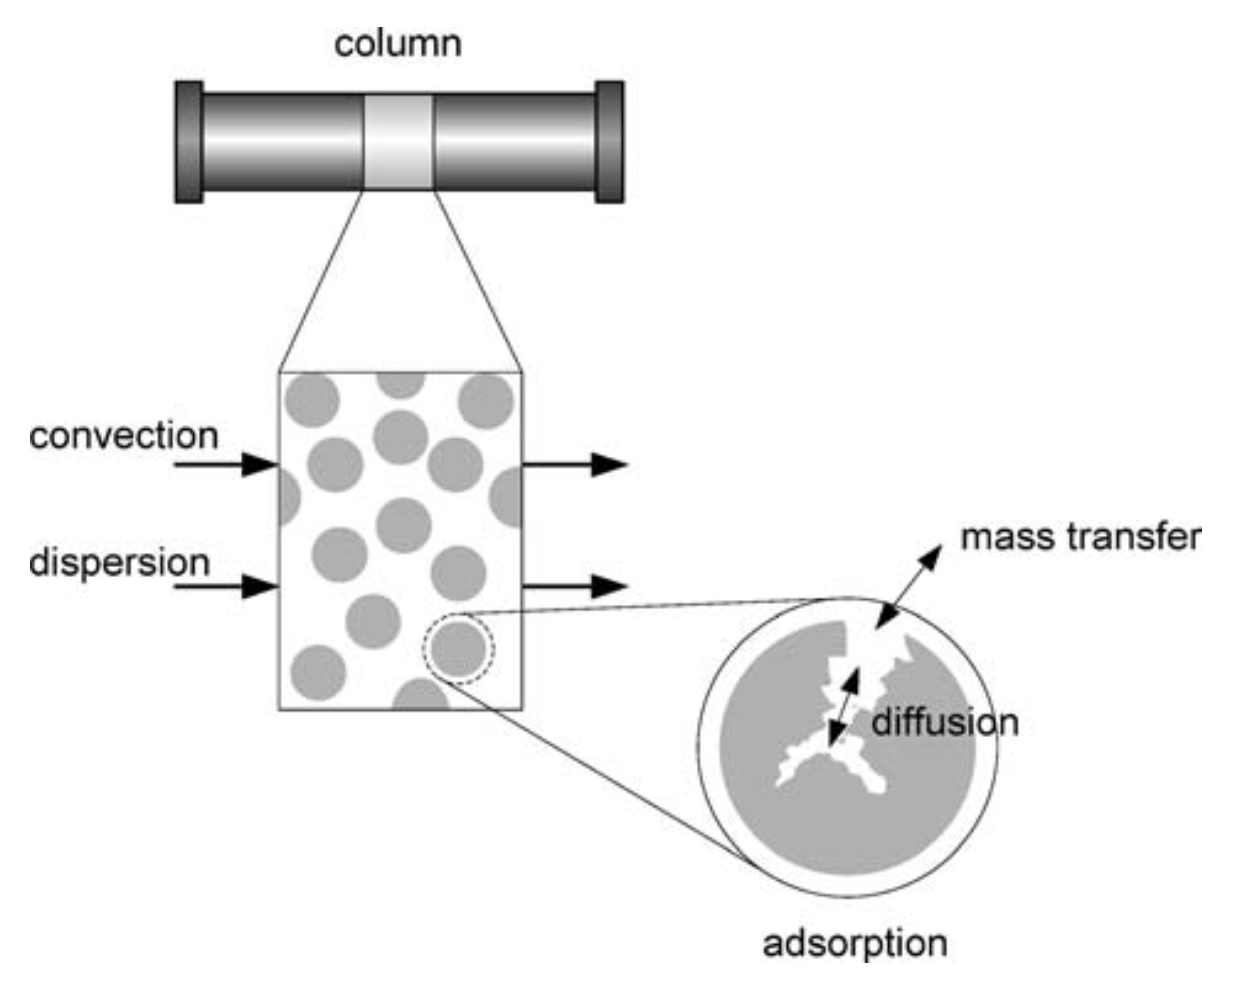
\includegraphics[width=0.55\textwidth]{diagramtransport.png}
\caption{Effects considered in chromatography model. Taken from Smith XX}
\end{figure}

\begin{itemize}
\item convection
\item Dispersion
\item Pore diffusion
\item Surface diffusion
\item adsorption kinetics
\item mass transfer from the mobile phase into the boundary layer of the stationary phase
\end{itemize}

In modeling liquid chromatographic processes, frequently different assumptions can be justified which lead to simplification in the mathematical models. The simplest model, known as the ideal model, neglects dispersion, pore and surface diffusion and mass transfer effects. On the other extreme, the most accurate model, known as the General Rate Model (GRM), consider all the phenomena listed above. In between, several models have been introduced in literature and are known as lumped transport models. Figure XX shows a basic diagram with a high-level classification of chromatography models and its corresponding variables.

\begin{figure}[h]
\centering
\label{cmodels}
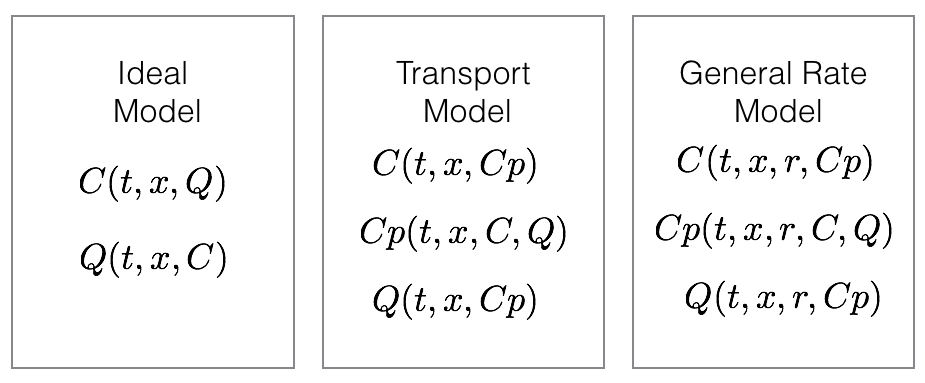
\includegraphics[width=0.75\textwidth]{models.png}
\caption{High-level classification of chromatography models}
\end{figure}

Where $C$ represents the concentration vector of all species in the mobile phase, $Cp$ the concentration vector of all species in the pores of the absorbent particles, and $Q$ the concentration vector of species in the particles, also known as loadings. The ideal model takes into account only convective transport and thermodynamics. This model neglects the influence of axial dispersion and all mass transfer effects. Consequently, the loadings and concentrations within the absorbent particles are assumed to be constant and not a function of the particle radius. Furthermore, the concentration in the mobile phase is identical to the concentration in the particle pores. Therefore, for each chemical species in the chromatography column the ideal model introduces two equations

\begin{align}
& \frac{\partial C}{\partial t} = \left(\frac{\epsilon-1}{\epsilon}\right) \frac{\partial Q}{\partial t}-v\frac{\partial C}{\partial x} \\
& a \frac{\partial Q}{\partial t} = f_{\text{ads}}(C,Q)
\end{align}

The first equation corresponds to a mass balance in the mobile phase and the second equation to an isotherm that describes the adsorption in the adsorbent particles. The initial conditions for the concentration and
the loading generally assume zero values and the inlet boundary condition is commonly represented as a piecewise polynomial

\begin{align*}
&C(0,x) = 0\\
&Q(0,x) = 0\\
&C(t,x=0) = c_{\text{in}}(t)\\
\end{align*}

A common condition for inlet function is a rectangular pulse or a step function. The ideal model is very often extended to account for dispersive effects by lumping all band broadening effects into a dispersion coefficient.

\begin{align}
& \frac{\partial C}{\partial t} = \left(\frac{\epsilon-1}{\epsilon}\right) \frac{\partial Q}{\partial t}-v\frac{\partial C}{\partial x} + D\frac{\partial^2C}{\partial x^2}\\
& a \frac{\partial Q}{\partial t} = f_{\text{ads}}(C,Q)
\end{align}

The next level of detail in the model hierarchy of Figure \ref{cmodels} is the so called Transport models. This model considers adsorption equilibrium, convection, mass transfer and band broadening. Therefore, it involves one more vector of variables that accounts for the mass transfer phenomena in the adsorption particles. For derivations and details of transport models the reader can refer to Schmidt et al (2012) and Guiochon et al. (2006). 

\begin{align}
& \frac{\partial C}{\partial t} = -v\frac{\partial C}{\partial x} + D\frac{\partial^2C}{\partial x^2} \\
& \frac{\partial C_p}{\partial t} = \left(\frac{\epsilon-1}{\epsilon}\right) \frac{\partial Q}{\partial t} + k_{eff}(C-C_p)\\
& a \frac{\partial Q}{\partial t} = f_{\text{ads}}(C_p,Q)
\end{align}

Finally, the most accurate model in the hierarchy of Figure \ref{cmodels} is the general rate model. GRMs are among the most detailed continuous models considered in literature. The underlying equations in the GRM combine
mass transfer in the liquid film and inside the pores as well as surface diffusion and adsorption kinetics in various kinds. 

\begin{align}
& \frac{\partial C}{\partial t} = -v\frac{\partial C}{\partial x} + D\frac{\partial^2C}{\partial x^2} -  \left(\frac{\epsilon-1}{\epsilon}\right) k_f(C-C_p(:,:,r_p))\\
& \frac{\partial C_p}{\partial t} = D_p\left(\frac{\partial^2C_p}{\partial r^2} + \frac{2}{r} \frac{\partial C_p}{\partial r}\right) -  \left(\frac{\epsilon-1}{\epsilon}\right)\frac{\partial Q}{\partial t}\\
& a \frac{\partial Q}{\partial t} = D_{ps}\left(\frac{\partial^2Q}{\partial r^2} + \frac{2}{r} \frac{\partial Q}{\partial r}\right) + f_{\text{ads}}(C_p,Q)
\end{align}

Further details on GRMs can be found in Guiochon et al. (2006) and Lieres and Andersson, 2010.

\section{Numerical solution of chromatography models}

The model equations described in the previous section include space and time derivatives. Independently of the chromatography model used, simulating a chromatography column involves solving a system of partial differential equations. For preparative chromatography the models usually involve highly nonlinear isotherms that couple with the PDEs constitute a PDAEs. In general the solution of nonlinear PDAEs is not achievable by means of analytical methods and hence it must be obtained numerically. The numerical solution can be obtained either by using self-developed programs or commercially available dynamic process simulation tools.
\\
\\
In general the numerical solution procedure involves the following
steps:

\begin{enumerate}
\item Transformation of the PDAE system into a set of differential algebraic equations (DAE) with respect to time by discretization of the spatial derivatives. Several discretization techniques can be applied to discretize the spacial domain. Examples of this techniques are finite volumes, finite elements and finite differences. While the latter is a simple numerical procedure that can be directly applied to any model, it suffers from inaccuracy and it may run into instability problems. Finite volumes, on the other hand, may provide more accurate results and more stability. 
\item Solving the DAEs using numerical integration routines, which can involve another discretization into a nonlinear algebraic system (NLA) or a invoking an adaptive step integrator that can integrate the (DAE) in time. Among the various numerical techniques for discretizing the time domain and reducing the DAE into an NLA, the finite element method has proven to be very efficient. This discretization method can be used for systems with stiff gradients. On the other hand, an adaptative integration approach benefits from the fact that it requires less memory usage, as it solves a smaller NLA in each time step, but more importantly it do not require a good initial guess for every point in the time trajectory.
\end{enumerate}

The software packages currently available for modeling chromatography columns 
present a variety of alternatives to execute the two steps listed above. Some software packages approach the problem with a complete discretization of space and time while others follow a method of lines to get a solution. Table XX summarizes different packages that efficiently solve chromatography models with optimal routines in highly efficient programming languages like C, C++, or fortran. However, a flexible package that would allow users to experiment with different methodologies seem to be not available. The excellent performance of packages like the ones listed in Table XX comes at the price of "inextensibility" and "inflexibility" since only skillful programmers acquainted with low level programming languages can actually dig into the code to extend it and modified. A chromatography package written in an interpreter language, like Python or R, would be easier to extend as more users would have the skills require to modify and extend the code. However, a package like that would lack the computational efficiency that other packages enjoy. Given the raising popularity of Python, and its flexibility to drive programs written in other languages, an excellent alternative would be to drive chromatography modeling from python by constructing models in python and solving the PDAE system of equations with efficient languages written in low level languages. 
\begin{figure}[h]
\label{software}
\centering
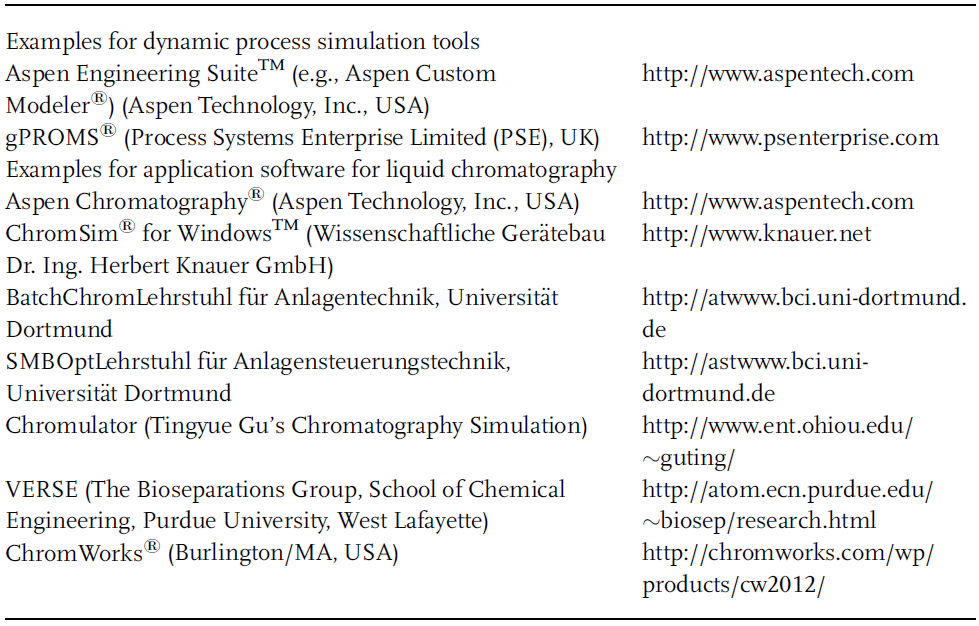
\includegraphics[width=\textwidth]{software.png}
\caption{Chromatography modeling packages. Taken from Schmidt (2012)}
\end{figure}
For all of the reasons listed above we have created pychrom, a python package for modeling and optimization of chromatography columns. As will be described in the next section, the package was design for easy extensibility and efficient modeling/optimization of chromatography columns.


\section{Pychrom: Python package for chromatography modeling and optimization}

Pychrom supports an object-oriented design for the definition of chromatography models. The basic steps of a simple modeling process are:

\begin{enumerate}
\item Create model and declare components

\item Invoke solver (CADET, IPOPT, CASADI)

\item Query results
\end{enumerate}

The design features of the pychrom package revolve around the need to have different "modellers" for the same "model". A model is an abstraction of a chromatography process. A modeller is the implementation of that abstraction in a particular engine or solver. At the time of writing there are two modellers: CADET and Pyomo. The former uses MOL+IVP strategy to solve the PDAE system. The latter uses a NLA (full discretization) strategy. This project aims at providing an abstration that allows the definition of a model in an abstract way, and the implementation (or interpretation) of that model in different modellers, in order to enable the comparison and contrasting of alternative modeling approaches for simulation and optimization.

\begin{figure}[!h]
\label{objects}
\centering
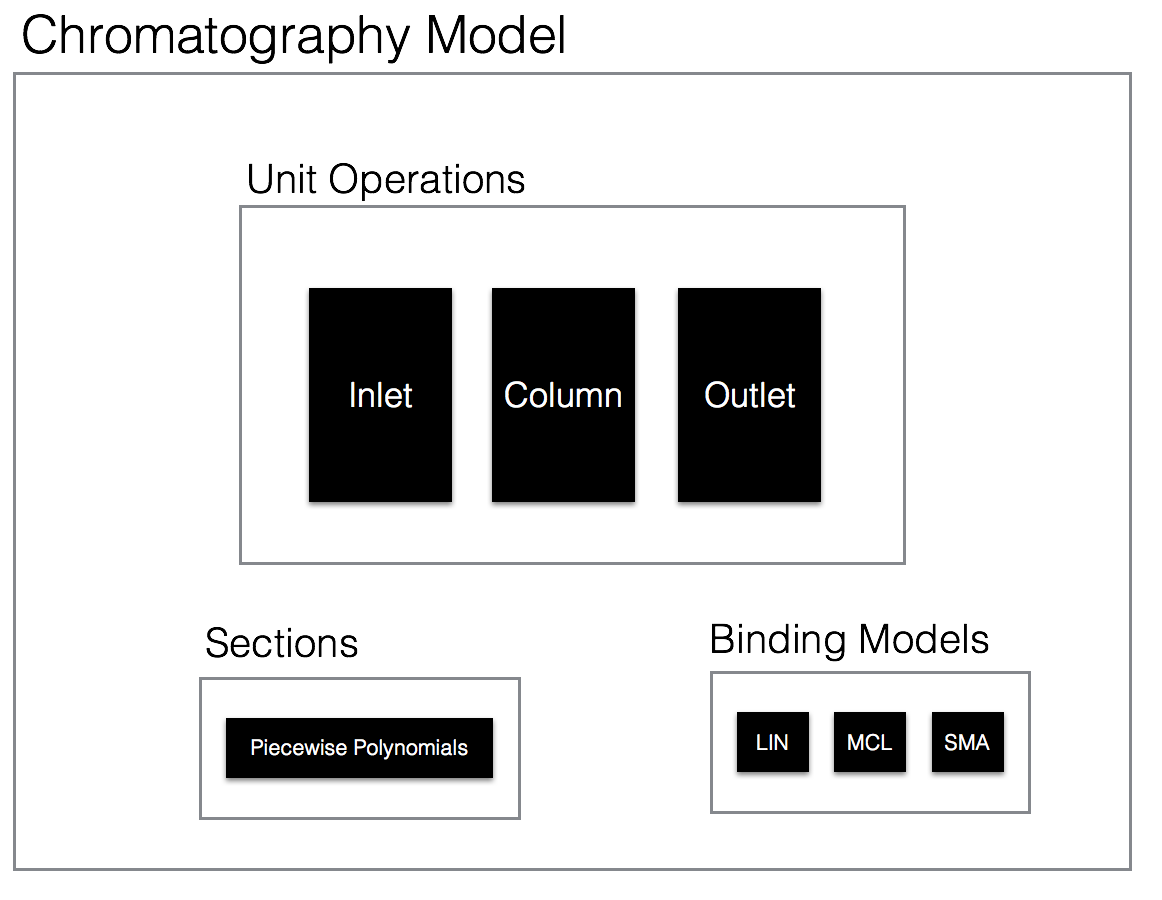
\includegraphics[width=\textwidth]{boxes.png}
\caption{Model components}
\end{figure}

In pychrom the simulation of a chromatography column can be done very efficiently. A chromatography model is built in python as a collection of python objects declare within the core module of pychrom. The abstraction of a model as a collection of objects is exemplified in Figure \ref{objects}. To create a model one must define a chromatography model object and then attach different components to it. The model needs to have at least two unit operations, and inlet and a column. The inlet can have different sections, which represent the piecewise polynomials that define the inlet boundary conditions described in section 2. Similarly a column must have an isotherm that defines the kinetics or thermodynamics of the adsorption. The current implementation supports 3 different isotherms (binding models); linear (LIN), multi-component langmuir (MCL), and steric mass action (SMA). Details on the implementation of the classes can be found in the UML diagram attached in the appendix. All classes are design following an inheritance scheme that facilitates adding new components with few effort (e.g. other binding models).  
\\
\\
Once the model has been created it can be sent to a efficient solver like CADET or IPOPT. Both solvers written in C++, will perform all intensive computations and exploit the high performance computing advantages of the low level programming language. On one hand, The Chromatography Analysis and Design Toolkit, CADET, will take the model, discretize space and invoke the Sundials integrator IDAS for solving the DAE. Alternatively, the chromatography model can be given to PYOMO to discretize space and time and give the NLA to IPOPT to solve it. All the results are latter parsed and loaded into xarrays for easy post-processing in python. This will make accessible all concentrations of different species at every location and time. The advantage of having this data in python is that any submodule available in python can be used for post-processing. For example, one can easily use subroutines in scipy to put together a parameter estimation problem and try different methods to fit data. Additionally, one can use python interactive modules like plotly to visualize and interact with the data. Note that all this features would not be easily accessible at a lower programming level (C, C++) but python facilitates any computational experiment. 
\\
\\
An example of how to create and simulate a chromatography model in pychrom is as follows:

\lstinputlisting[language=Python]{examplelin.py}

All data is declare in an object oriented fashion and objects are attached to a chromatography model object. Running that script produces the following output 

\begin{figure}[!h]
\label{objects}
\centering
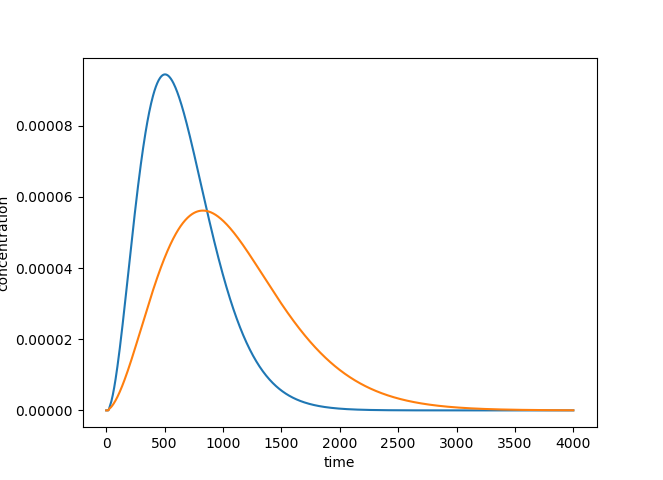
\includegraphics[width=0.7\textwidth]{example1.png}
\caption{Example 1}
\end{figure}

For models with several species, data can be parsed from a yaml file instead of being explicitly defined in the python script.

\lstinputlisting[language=Python]{examplesma.py}

\begin{figure}[!h]
\label{objects}
\centering
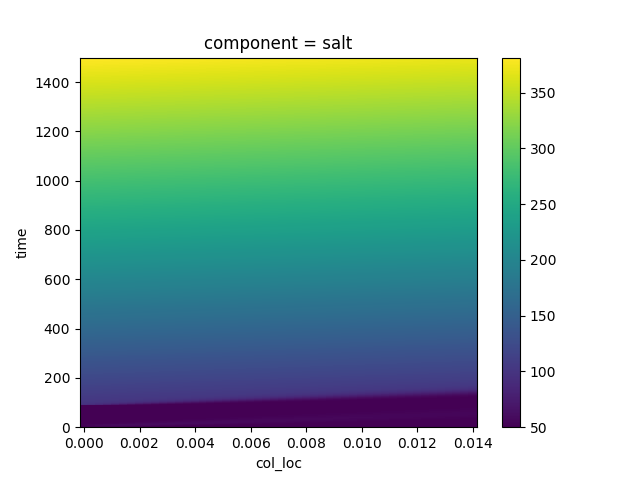
\includegraphics[width=0.7\textwidth]{example2a.png}
\caption{Example 2a}
\end{figure}

\begin{figure}[!h]
\label{objects}
\centering
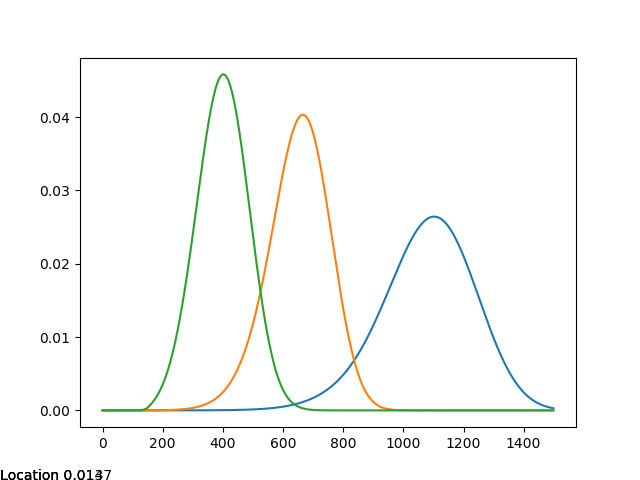
\includegraphics[width=0.7\textwidth]{example2b.png}
\caption{Example 2b}
\end{figure}

Now to see the advantage driving the modeling from python lets consider the case where we want to run several simulations with stochasticity in some of the parameters. After all simulations are finished we gather the data and determine the average retention time of each species in the system. This task can be easily done with pychrom and with few effor we can even run the simulations in parallel with the mpi4py module in python. 
\\
\\
First, on one script we create the model and define a function to determine the retention time.

\lstinputlisting[language=Python]{pychrom_example.py}

Then we build different instances with stochasticity in the parameters on different processors and use mpi to gather the results and compute the average residence time.

\lstinputlisting[language=Python]{mpi_pychrom.py}

In conclusion, driving the chromatography modeling from python open several possibilities to improve our analysis of chromatography results. We are particularly interested in driving an optimization with an interior point method as we will describe in the following section.

\section{Optimization}
IN PROGRESS
%%% End document
\end{document}